\documentclass[12pt]{article}
\usepackage{lipsum}
\usepackage{epigraph}
\usepackage{graphicx}
\usepackage[swedish]{babel}
\usepackage{natbib}
\usepackage[utf8]{inputenc}
\usepackage[margin=0.5in, bmargin=0.8in]{geometry}

\usepackage{csquotes}

\begin{document}
\title{Kandidatarbete i elektroakustisk komposition\\(arbetstitel)}
\author{Karl Johannes Jondell}

\maketitle

\begin{abstract}
Vad handlar detta projekt om?

Vem är detta projekt för? Vem kommer läsa denna text? 
\end{abstract}

\begin{keyword}
sonifiering, diabetes, interaktion
\end{keyword}

\tableofcontents

\section{Introduktion}
Projekt...

\subsection{Bakgrund}
Projekt från ettan, diabetes-synth, radiostation, etc.
Pandemin....

\section{Sonifiering: vad är det?}
sonifiering... \cite{bijsterveld_sonic_2019}

Bearbetad data och orginaldata. Sensorfel.

\section{Diabetes}
Inte vara ensam i sin sjukdom... (utveckla)

Dela med sig av sina värden (t.ex. i olika grupper) men utan nån värdering/stigmatisering...

\section{Deltagande och interaktion}
Erfarenheter från projekt i ettan. Delande.

\subsection{\emph{Data mining} och integritet}
Problem i ett sådant projekt med GDPR och insamlande av så personlig data. Vem är jag att be om så pass personlig information som blodsockervärden? Offentligt vs. privat-projekt. (Tack vare projektet samrörelse med statlig myndighet? dvs. KMH, ett förtroendeingivande)

\section{Musiken}
Den konstnärliga friheten. Hur pass mycket kontroll som överlåtes till \enquote{serien} (i detta fall blodsockervärdet). Behöver musiken gestalta, spegla, estetisera erfarenheten som diabetiker? Eller vara intresseväckande, tillgänglig, \enquote{relaterbar}? 

\subsection{Rumslighet}
En \enquote{kör} av blodsockervärden, spatialiserade i nån mening för att ge en känsla av påverkan eller åverkan på musiken. 

Rumsligheten i ett sådant hyperdigitalt projekt som detta (...)

Konsertupplevelse (i Lilla salen? spela ett utdrag ur liveströmmen...)

\subsection{Temporalitet}
Den tidsmässiga uppfattningen av musiken. En 24/7 livestream av musiken (hur utgörs lyssnadet? formen? \emph{Slow as possible}, \emph{Longplayer} och liknande...)

\subsection{Generativt}
Musiken är generativ. Serialism?

\section{System}
\begin{figure}[h!]
\centering
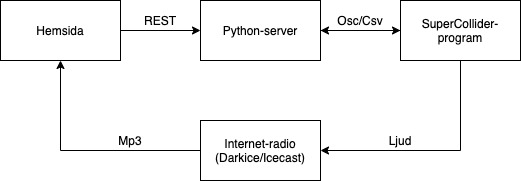
\includegraphics{../kod/Flowchart-program.jpg}
\caption{Flödesdiagram av system}
\end{figure}

\bibliographystyle{agsm}
\bibliography{bibtex/kandidatarbete.bib}

\end{document}

